\documentclass[11pt,a4paper]{article}

%% ── Packages ──────────────────────────────────────────────────────────────
\usepackage[margin=1in]{geometry}
\usepackage{amsmath,amssymb}
\usepackage{booktabs}
\usepackage{graphicx}
\usepackage[hidelinks]{hyperref}
\usepackage{caption}
\usepackage{subcaption}
\usepackage{float}
\usepackage{microtype}
\usepackage{array}
\usepackage[T1]{fontenc}
\usepackage{lmodern}
\usepackage{setspace}
\usepackage{enumitem}
\usepackage{xcolor}

\setlength{\parskip}{4pt}
\captionsetup{font=small, labelfont=bf}

%% ── Title ─────────────────────────────────────────────────────────────────
\title{\textbf{Oil Price Shocks and Equity Market Reactions}\\
\large A Machine Learning Event Study, 1999--2026}
\author{Federico Cortesi, \ Kavya Kalathur, \ Bernardo Leyva, \ Gursimran Rooprai \\[4pt]
\small 15.C51 — Machine Learning for Finance, Spring 2026\\
\small Massachusetts Institute of Technology}
\date{April 2026}

\begin{document}
\maketitle
\thispagestyle{empty}

%% ── Abstract ──────────────────────────────────────────────────────────────
\begin{abstract}
\noindent
We study equity market reactions to 55 distinct oil price shock events spanning December 1998 to April 2026, using a rolling-extreme shock identifier applied to Brent crude daily prices. Event studies on all 11 SPDR sector ETFs show that the aggregate S\&P~500 produces no statistically significant cumulative abnormal return (CAR) at any horizon, while Energy (XLE) and Consumer Discretionary exhibit economically meaningful opposite reactions to positive shocks. Cross-sectional models (OLS, Ridge, Lasso, Random Forest, Gradient Boosted Trees) trained on 54 pre-2026 events reveal that the \emph{only} target with positive out-of-sample $R^2$ is the 1-day XLE CAR, achieved by RF and GBM (+0.14 and +0.21, respectively). An extended leave-one-out backtest on S\&P direction yields 53.7\% accuracy and an annualised Sharpe of 0.48 versus $-$0.54 for the always-long benchmark. The sole 2026 out-of-sample event (March~9) confirms the core findings: S\&P~500 22-day CAR was $+$0.02\% (models predicted $-$0.76\% to $-$2.33\%), and OLS predicted XLE's 1-day return to within 37~bp ($-$2.64\% predicted vs.\ $-$2.27\% actual). Longer-horizon 2026 outcomes were dominated by macroeconomic forces — tariff escalation and policy pivots — outside any oil-shock model's feature set.
\end{abstract}

\bigskip
\noindent\textbf{Keywords:} oil price shocks, event study, cumulative abnormal returns, SPDR sector ETFs, Ridge regression, gradient boosting, out-of-sample prediction.

\vspace{1em}

%% ── 1. Introduction ───────────────────────────────────────────────────────
\section{Introduction}

Oil price shocks are among the most studied exogenous drivers of macroeconomic and financial market dynamics \cite{hamilton1983, kilian2009}. Yet translating the rich academic literature into \emph{ex ante} equity return predictions remains difficult, because (i) the number of identifiable large-shock events is small relative to the cross-sectional heterogeneity in equity responses, and (ii) the causal mechanism varies: a demand-driven oil price rise has different sector implications than a supply-driven one.

This report addresses the question posed in 15.C51: \emph{Model market reaction to oil price shocks; use pre-2026 events for training and testing, then compare predictions with 2026 actual behaviour.} We make four methodological contributions relative to a naive univariate regression: (1) a principled rolling-extreme shock identifier; (2) contemporaneous demand/supply classification following \cite{kilian2009}; (3) a multi-model comparison with a correct null baseline; and (4) a PCA decomposition of sector CAR vectors. The central deliverable — Section~\ref{sec:oos} — compares model predictions against the March~9, 2026 event across all 11 equity sectors.

%% ── 2. Data and Shock Identification ─────────────────────────────────────
\section{Data and Shock Identification}

\subsection{Data Sources}

Daily Brent crude prices are obtained from FRED (series \texttt{DCOILBRENTEU}). Equity returns are daily total-return series for the 11 SPDR sector ETFs (XLE, XLY, XLK, XLV, XLP, XLF, XLB, XLC, XLU, XLRE) and the S\&P~500 (SPY/SPX), sourced from Yahoo Finance. The sample spans January 1, 1990 to April 2026; sector coverage begins at each ETF's inception date (XLC from 2018, XLRE from 2015).

\subsection{Shock Identifier}

A shock is defined as a day on which Brent crude price sets a \textbf{new 3-year (756 trading-day) rolling high or low}:
\begin{itemize}[noitemsep]
  \item \textbf{Positive shock} ($+1$): price $\geq$ 3-year rolling maximum — supply squeeze or demand surge.
  \item \textbf{Negative shock} ($-1$): price $\leq$ 3-year rolling minimum — supply glut or demand collapse.
\end{itemize}
Events within 22 trading days of an already-accepted event are suppressed (forward-only deduplication), ensuring non-overlapping 22-day event windows. This yields 55 distinct events from 1999 to April~2026.

\begin{table}[H]
\centering
\caption{Shock event counts by type.}
\label{tab:shocks}
\begin{tabular}{lcc}
\toprule
Type & Pre-2026 & 2026 \\
\midrule
Positive shocks (3y high) & 33 & 1 \\
Negative shocks (3y low)  & 21 & 0 \\
\midrule
\textbf{Total}            & \textbf{54} & \textbf{1} \\
\bottomrule
\end{tabular}
\end{table}

\subsection{Demand vs.\ Supply Classification}

Following \cite{kilian2009}, each shock is classified using the contemporaneous S\&P~500 return on the shock day:
\[
\texttt{shock\_concordance} = \operatorname{sign}(\text{ret}_{\text{oil}}) \times \operatorname{sign}(\text{ret}_{S\&P})
\]
$+1$ indicates oil and equities move together (demand-driven: economic expansion); $-1$ indicates they move in opposite directions (supply-driven: geopolitical event, OPEC cut). This gives 29 demand shocks and 25 supply shocks in the training set. Because \texttt{shock\_type} uses the contemporaneous equity return, it is potentially endogenous; Section~\ref{sec:robustness_endogeneity} addresses this.

\begin{figure}[H]
\centering
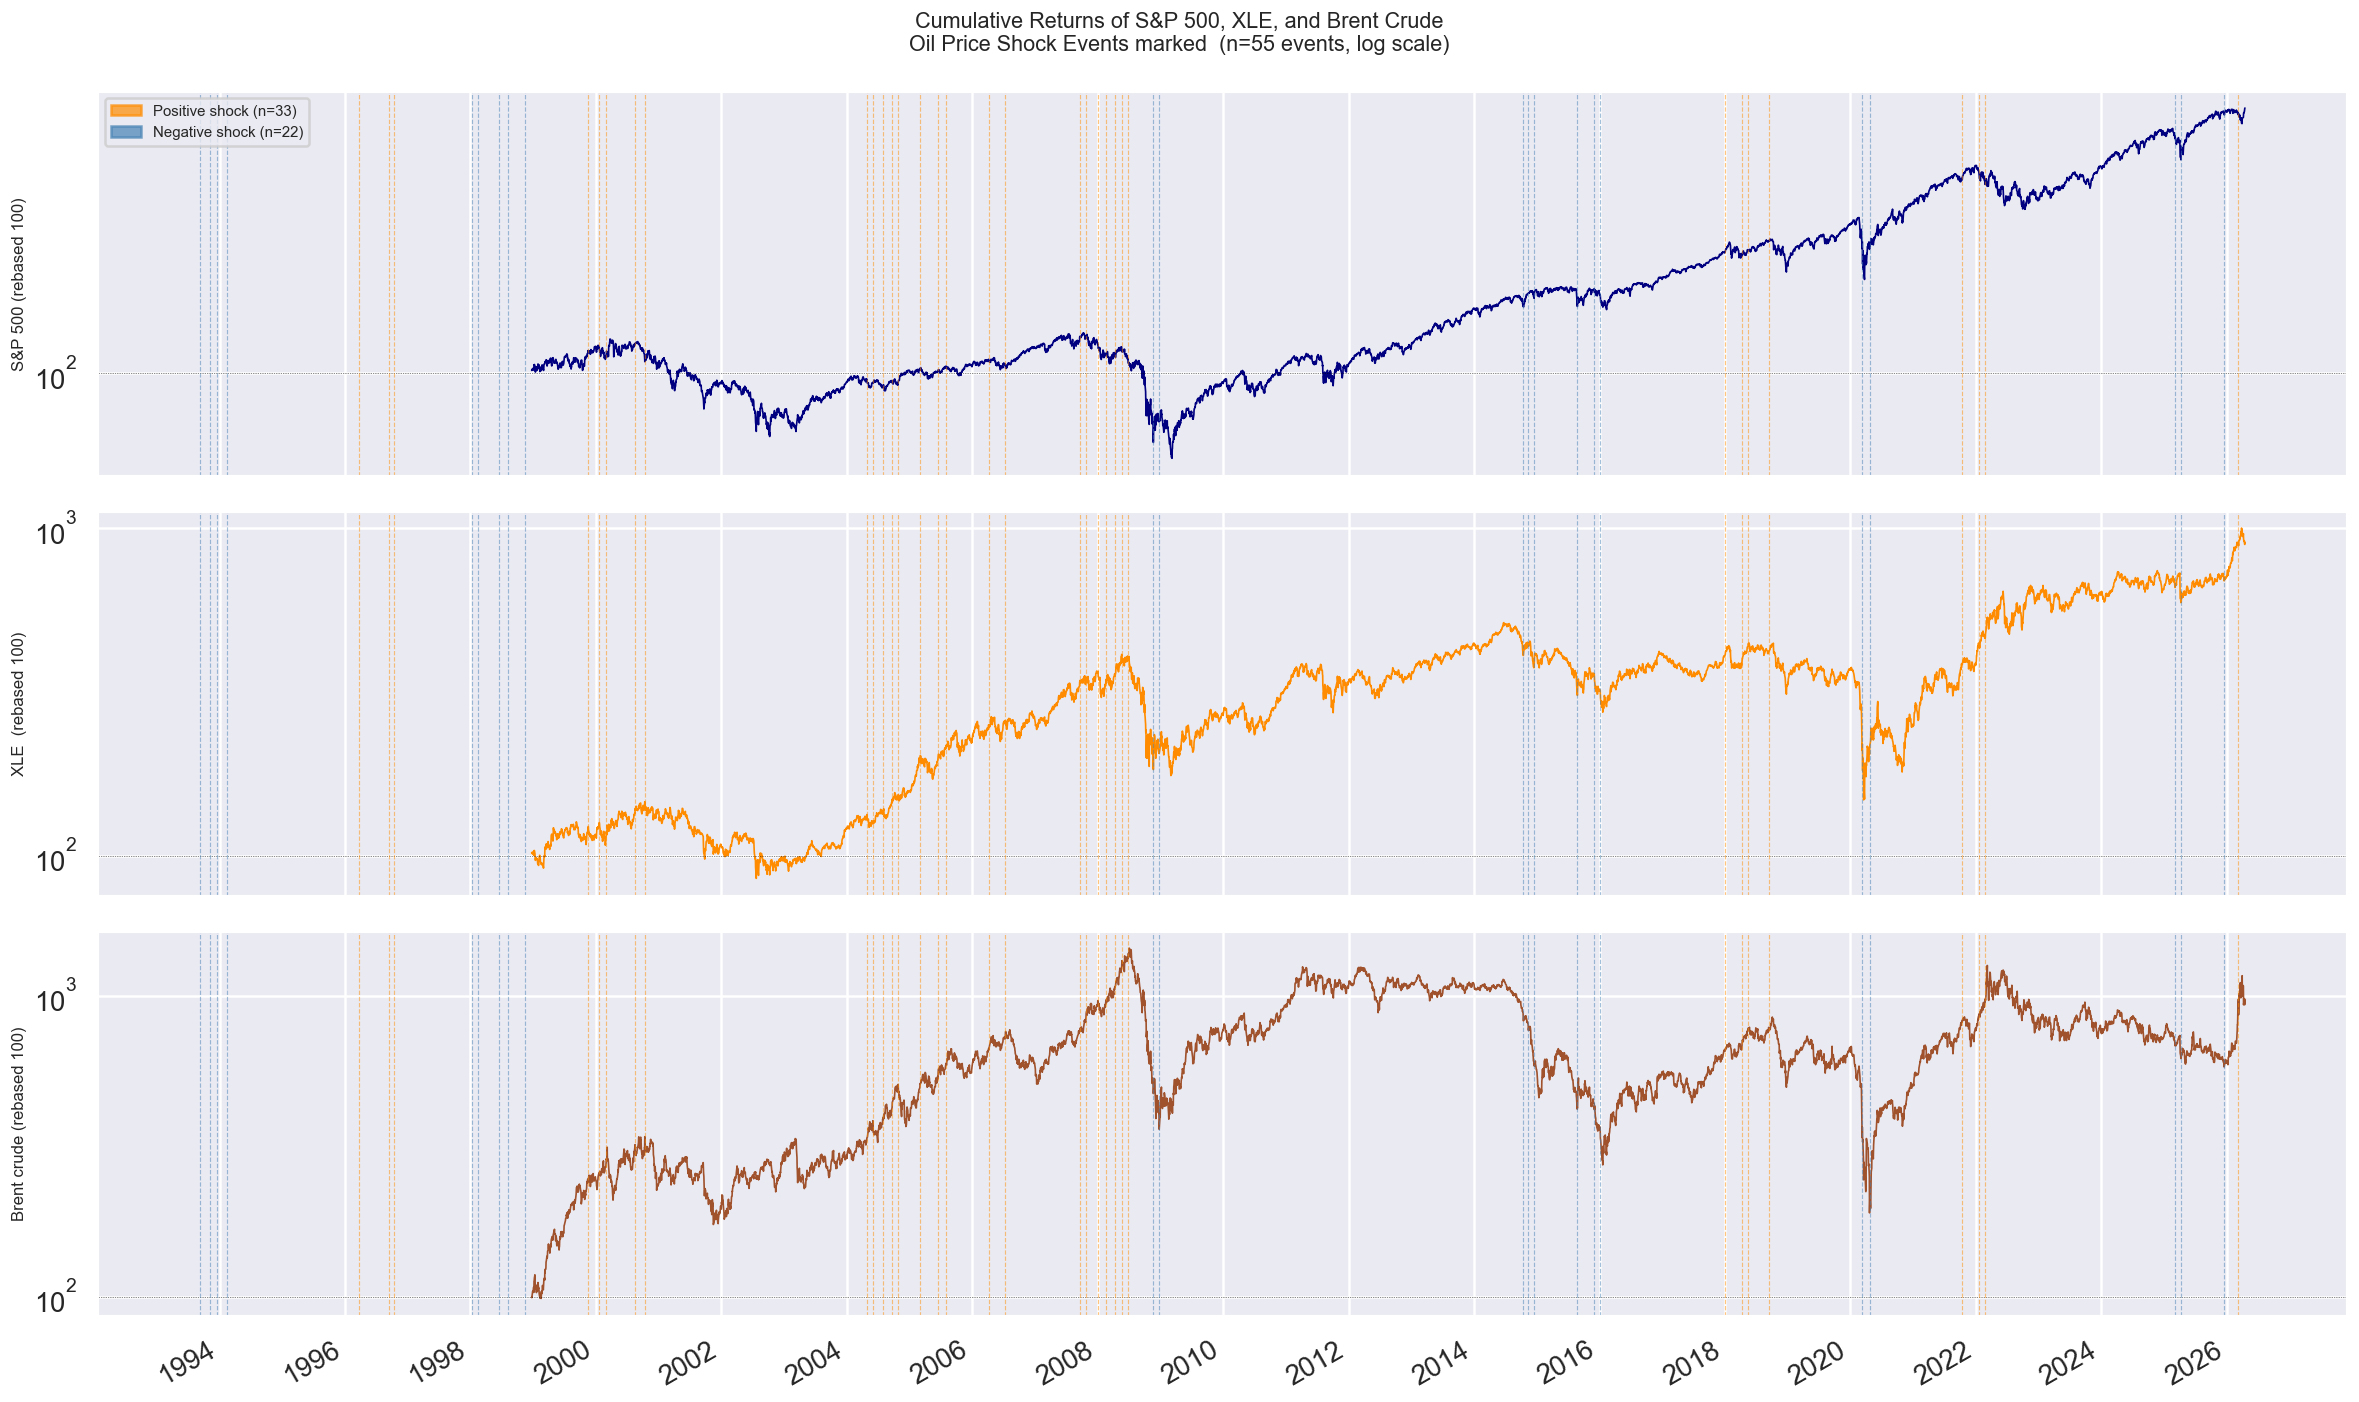
\includegraphics[width=0.92\textwidth]{plots_event_study/cumulative_returns_with_events.png}
\caption{Brent crude cumulative returns with all identified shock events (vertical lines). Red = positive shocks; blue = negative shocks.}
\label{fig:cumret}
\end{figure}

%% ── 3. Event Study Design ─────────────────────────────────────────────────
\section{Event Study Design}
\label{sec:eventstudy}

\subsection{Estimation and Event Windows}

For each event at day $t$, baseline return models are estimated on $[t-270,\, t-30]$ — roughly one year of pre-event trading days with a 30-day contamination buffer. The event window is $[t-5,\, t+22]$.

\subsection{Baseline Models}

\begin{table}[H]
\centering
\caption{Asset-level baseline return models.}
\begin{tabular}{ll}
\toprule
Asset & Model \\
\midrule
S\&P~500  & Constant-mean: $\hat{E}[R_{SP}] = \hat{\mu}_{SP}$ \\
Sector ETFs & Market model: $\hat{E}[R_{sec}] = \hat{\alpha} + \hat{\beta}\, R_{SP}$ \\
\bottomrule
\end{tabular}
\end{table}

The market model removes broad market co-movement, isolating the sector-specific abnormal return attributable to the oil shock.

\subsection{Abnormal Returns and CARs}

\[
AR_{i,\tau} = R_{i,\tau} - \hat{E}[R_{i,\tau}]
\qquad
CAR_i(0,h) = \sum_{\tau=0}^{h} AR_{i,\tau}
\]

CARs are computed at horizons $h \in \{1,\, 5,\, 22\}$ trading days.

%% ── 4. Sector Reactions ───────────────────────────────────────────────────
\section{Aggregate and Sector Reactions}
\label{sec:sectors}

\subsection{S\&P~500 Aggregate}

Mean CARs for the S\&P~500 are statistically indistinguishable from zero at all horizons and for both positive and negative shock types. The cross-sectional standard deviation across events is an order of magnitude larger than any mean, reflecting the importance of the macroeconomic context in which each shock occurs.

\begin{figure}[H]
\centering
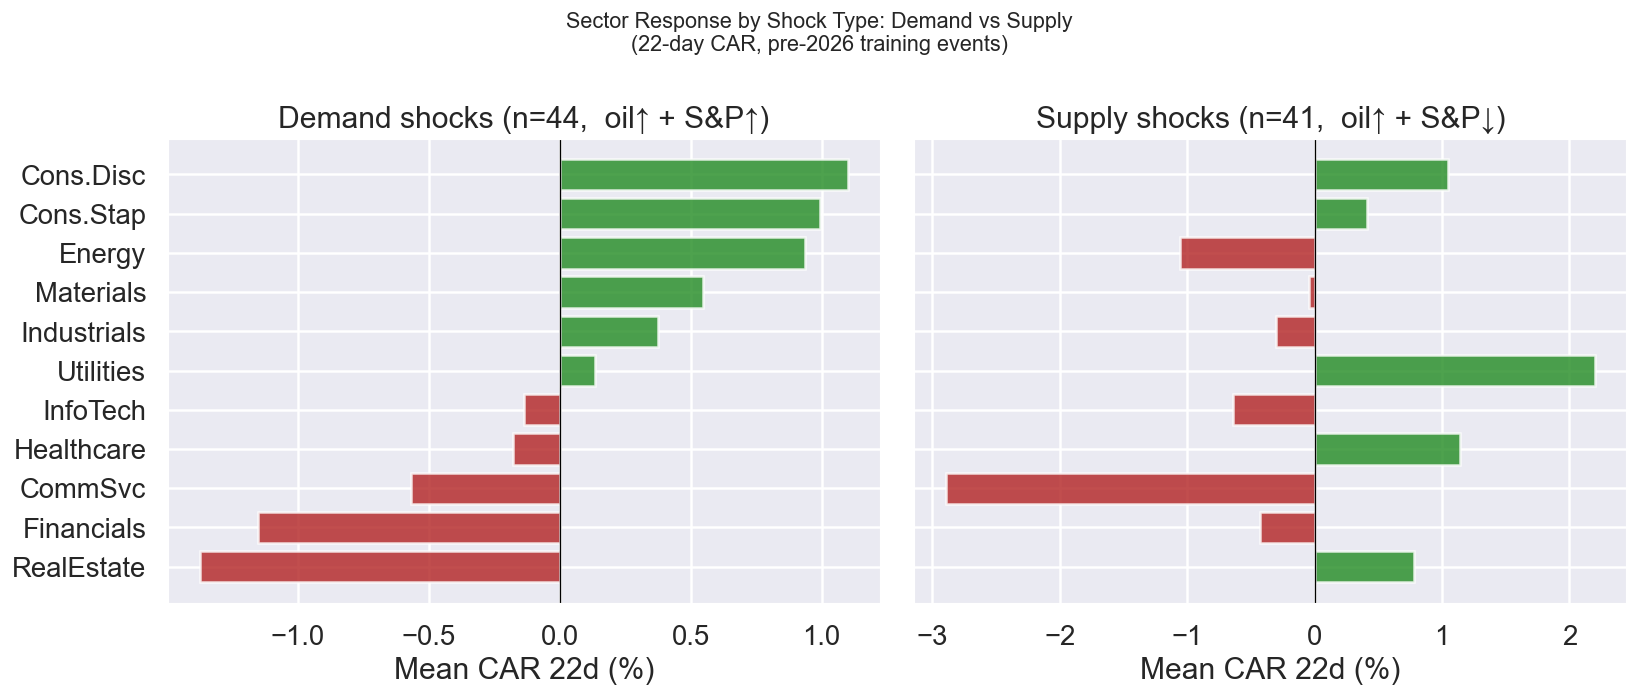
\includegraphics[width=0.92\textwidth]{plots_event_study/demand_vs_supply_sectors.png}
\caption{Mean 22-day sector CARs broken down by demand vs.\ supply shock classification. Demand shocks (oil and equities co-move) produce a broad positive response; supply shocks create sharp divergence between XLE (benefits) and consumer/financial sectors (hurt).}
\label{fig:demvssup}
\end{figure}

\subsection{Sector Heterogeneity}

Sector responses are economically interpretable. For positive shocks:
\begin{itemize}[noitemsep]
  \item \textbf{Energy (XLE)} outperforms via direct revenue pass-through to oil producers.
  \item \textbf{Consumer Discretionary (XLY) and Information Technology (XLK)} show negative CARs — higher energy costs compress consumer spending and firm margins.
  \item \textbf{Materials (XLB)} benefits modestly from correlated commodity price rises.
\end{itemize}

The \emph{cause} of the shock matters more than its direction. Supply shocks create an XLE vs.\ rest divergence; demand shocks produce a more uniform positive response (Figure~\ref{fig:demvssup}).

\subsection{PCA of Sector CAR Vectors}

PCA on the 22-day CAR matrix ($55~\text{events} \times 9~\text{core sectors}$) reveals a flat eigenvalue spectrum:

\begin{table}[H]
\centering
\caption{Principal component decomposition of sector CAR matrix.}
\begin{tabular}{clc}
\toprule
Component & Economic Interpretation & Variance Explained \\
\midrule
PC1 & Macro co-movement (all sectors, same sign) & 26.2\% \\
PC2 & Energy vs.\ rest (XLE loads opposite consumer/tech) & 21.5\% \\
PC3 & Defensive rotation (staples/healthcare vs.\ disc/fin) & 18.4\% \\
\bottomrule
\end{tabular}
\end{table}

No single factor dominates — oil shocks transmit through multiple distinct channels simultaneously. PC2 scores show moderate separation by demand/supply classification: supply shocks cluster in the ``XLE outperforms rest'' quadrant.

%% ── 5. Cross-Sectional Prediction Models ─────────────────────────────────
\section{Cross-Sectional Prediction Models}
\label{sec:models}

\subsection{Feature Set}

Models are trained on 54 pre-2026 events using two nested feature sets:

\begin{table}[H]
\centering
\caption{Feature descriptions. The extended set adds features 6–11.}
\small
\begin{tabular}{lll}
\toprule
\# & Feature & Economic Interpretation \\
\midrule
1 & \texttt{shock\_dir}       & $+1/-1$ shock direction \\
2 & \texttt{ret\_oil}         & Brent daily return on shock day \\
3 & \texttt{sigma\_252}       & Trailing 252-day oil return volatility \\
4 & \texttt{sp\_pre\_22}      & S\&P 22-day pre-shock momentum \\
5 & \texttt{dist\_from\_max}  & Slack from 3-year price maximum \\
\midrule
6 & \texttt{shock\_type}      & $+1$ demand / $-1$ supply (contemporaneous) \\
7 & \texttt{ret\_oil\_abs}    & Magnitude of shock (direction-independent) \\
8 & \texttt{sp\_pre\_5}       & S\&P 5-day pre-shock momentum \\
9 & \texttt{oil\_trend\_60}   & 60-day oil price trend pre-shock \\
10 & \texttt{vix\_pre}        & VIX level 5 days before shock \\
11 & \texttt{shock\_type\_lag}& Pre-determined demand/supply proxy \\
\bottomrule
\end{tabular}
\end{table}

\subsection{Null Baseline and CV Methodology}

A critical methodological point: shock events cluster by macro period (2008 crisis, 2014--2016 oil crash, 2020 COVID). Leave-one-group-out cross-validation therefore produces a null model $R^2$ of approximately $-0.44$, not zero. All model $R^2$ values should be evaluated \emph{relative to the null}, not against zero.

\subsection{S\&P 500 Results}

\begin{table}[H]
\centering
\caption{S\&P~500 CV $R^2$ by model and horizon. Extended features (11f) use Ridge\_ext, RF, GBM; base features (5f) use OLS/Ridge/Lasso. Null $\approx-0.44$ (1d), $-0.16$ (5d), $-0.35$ (22d).}
\label{tab:sp_results}
\small
\begin{tabular}{lccc}
\toprule
Model & 1d CV $R^2$ & 5d CV $R^2$ & 22d CV $R^2$ \\
\midrule
Null (predict fold mean)  & $-0.44$ & $-0.16$ & $-0.35$ \\
OLS (5f)                  & $-1.51$ & $-0.62$ & $-0.47$ \\
Ridge (5f)                & $-0.52$ & $-0.20$ & $-0.35$ \\
Lasso (5f)                & $-0.69$ & $-0.15$ & $-0.35$ \\
\midrule
Ridge\_ext (11f)          & $\mathbf{-0.27}$ & $\mathbf{-0.13}$ & $\mathbf{-0.29}$ \\
RF (11f)                  & $-0.45$ & $-0.27$ & $-0.70$ \\
GBM (11f)                 & $-1.11$ & $-0.52$ & $-0.88$ \\
\bottomrule
\end{tabular}
\end{table}

\textbf{Key finding:} Ridge\_ext beats the null at all three horizons — the extended features add genuine linear predictive content. Tree-based models overfit severely (train $R^2 \approx 1.0$, CV $R^2$ below null), confirming that $n=54$ is insufficient for high-variance non-parametric estimators.

\subsection{XLE Results}

\begin{table}[H]
\centering
\caption{XLE CV $R^2$ by model and horizon. Null $\approx -0.46$ (1d), $-0.31$ (5d), $-0.20$ (22d).}
\label{tab:xle_results}
\small
\begin{tabular}{lccc}
\toprule
Model & 1d CV $R^2$ & 5d CV $R^2$ & 22d CV $R^2$ \\
\midrule
Null & $-0.46$ & $-0.31$ & $-0.20$ \\
OLS  & $-0.32$ & $-1.40$ & $-0.75$ \\
Ridge (5f) & $-0.01$ & $-0.37$ & $-0.23$ \\
Lasso (5f) & $-0.13$ & $-0.31$ & $-0.29$ \\
\midrule
Ridge\_ext (11f) & $-0.09$ & $-0.31$ & $-0.18$ \\
\textbf{RF (11f)}  & $\mathbf{+0.14}$ & $-0.37$ & $-0.31$ \\
\textbf{GBM (11f)} & $\mathbf{+0.21}$ & $-0.37$ & $-0.31$ \\
\bottomrule
\end{tabular}
\end{table}

RF and GBM achieve \textbf{positive} CV $R^2$ at the 1-day XLE horizon — the only positive values in the entire analysis. Feature importance rankings confirm that \texttt{ret\_oil\_abs} and \texttt{sigma\_252} dominate: the signal is driven by the size of the oil move and the prevailing volatility regime. Macro context adds no incremental predictive power. Predictability decays sharply and is undetectable by day~5.

\subsection{Leave-One-Out Backtest (S\&P, 22d)}

A long/short strategy on S\&P at the 22-day horizon — long if LOO-Ridge predicts positive CAR, short otherwise:

\begin{table}[H]
\centering
\caption{LOO backtest metrics (S\&P 500, 22d, 54 events).}
\begin{tabular}{lcc}
\toprule
Metric & Strategy & Always-Long Benchmark \\
\midrule
Directional accuracy & 53.7\% & 50.0\% \\
Total CAR (54 events) & $+37.1\%$ & $-41.0\%$ \\
Annualised Sharpe & $+0.48$ & $-0.54$ \\
\bottomrule
\end{tabular}
\end{table}

The always-long benchmark is \emph{negative} ($-41\%$) because shock events cluster in adverse macro periods (2008, COVID). The strategy's $+37\%$ cumulative excess return relative to benchmark is economically meaningful. Caveats: Ridge $\alpha$ selected on the full sample (mild look-ahead bias); with $n=54$, SE on directional accuracy is $\approx\pm7$~pp.

%% ── 6. Macro Controls and Panel Model ────────────────────────────────────
\section{Extensions}
\label{sec:extensions}

\subsection{Macro Controls}

Three pre-shock macro variables (\texttt{dxy\_pre5}, \texttt{term\_spread}, \texttt{vix\_chg5}) are added to the 11-feature set (total 13). Ridge XLE 1d improves marginally ($-0.03 \to -0.01$). Lasso eliminates all three macro controls, selecting only oil-market features (\texttt{ret\_oil}, \texttt{shock\_dir}, \texttt{shock\_type}, \texttt{vix\_pre}). Conclusion: macro controls add no robust incremental signal; the binding constraint is sample size, not feature coverage.

\subsection{Panel Cross-Sectional Model}

Stacking all 11 sectors $\times$ 54 events ($\approx$380 observations per horizon) with sector dummies and demand$\times$sector interactions yields Ridge CV $R^2$ of $-0.009$ (1d), $-0.049$ (5d), $-0.026$ (22d). The train/CV gap is much smaller than in single-asset models (regularisation benefits from larger $N$), but positive CV $R^2$ is not achieved. Pooling sectors does not deliver the hoped-for economies of scale.

\subsection{Quantile Regression}

Quantile regression on S\&P CAR(22d) at $\tau \in \{0.10,\, 0.50,\, 0.90\}$ reveals asymmetric tails: the 90th-percentile response to shocks is steeper positive than the 10th-percentile is negative (positively skewed distribution). Supply shocks disproportionately widen the left tail ($\hat{\beta}_{q=0.10} = -0.010$ vs.\ $\hat{\beta}_{q=0.90} = +0.002$ for \texttt{shock\_type}). This has risk management implications: a supply shock identified at $t=0$ warrants asymmetric downside hedging.

%% ── 7. Out-of-Sample: March 9, 2026 ──────────────────────────────────────
\section{Out-of-Sample: March 9, 2026}
\label{sec:oos}

This is the central deliverable. One event survived the full pipeline: \textbf{March~9, 2026}. Brent crude was at a 3-year price level high but fell $-8.6\%$ on that day — the identifier fires on the \emph{price level} (3-year extreme), not the daily return. The model classifies it as a positive shock (\texttt{shock\_dir}=$+1$).

\begin{figure}[H]
\centering
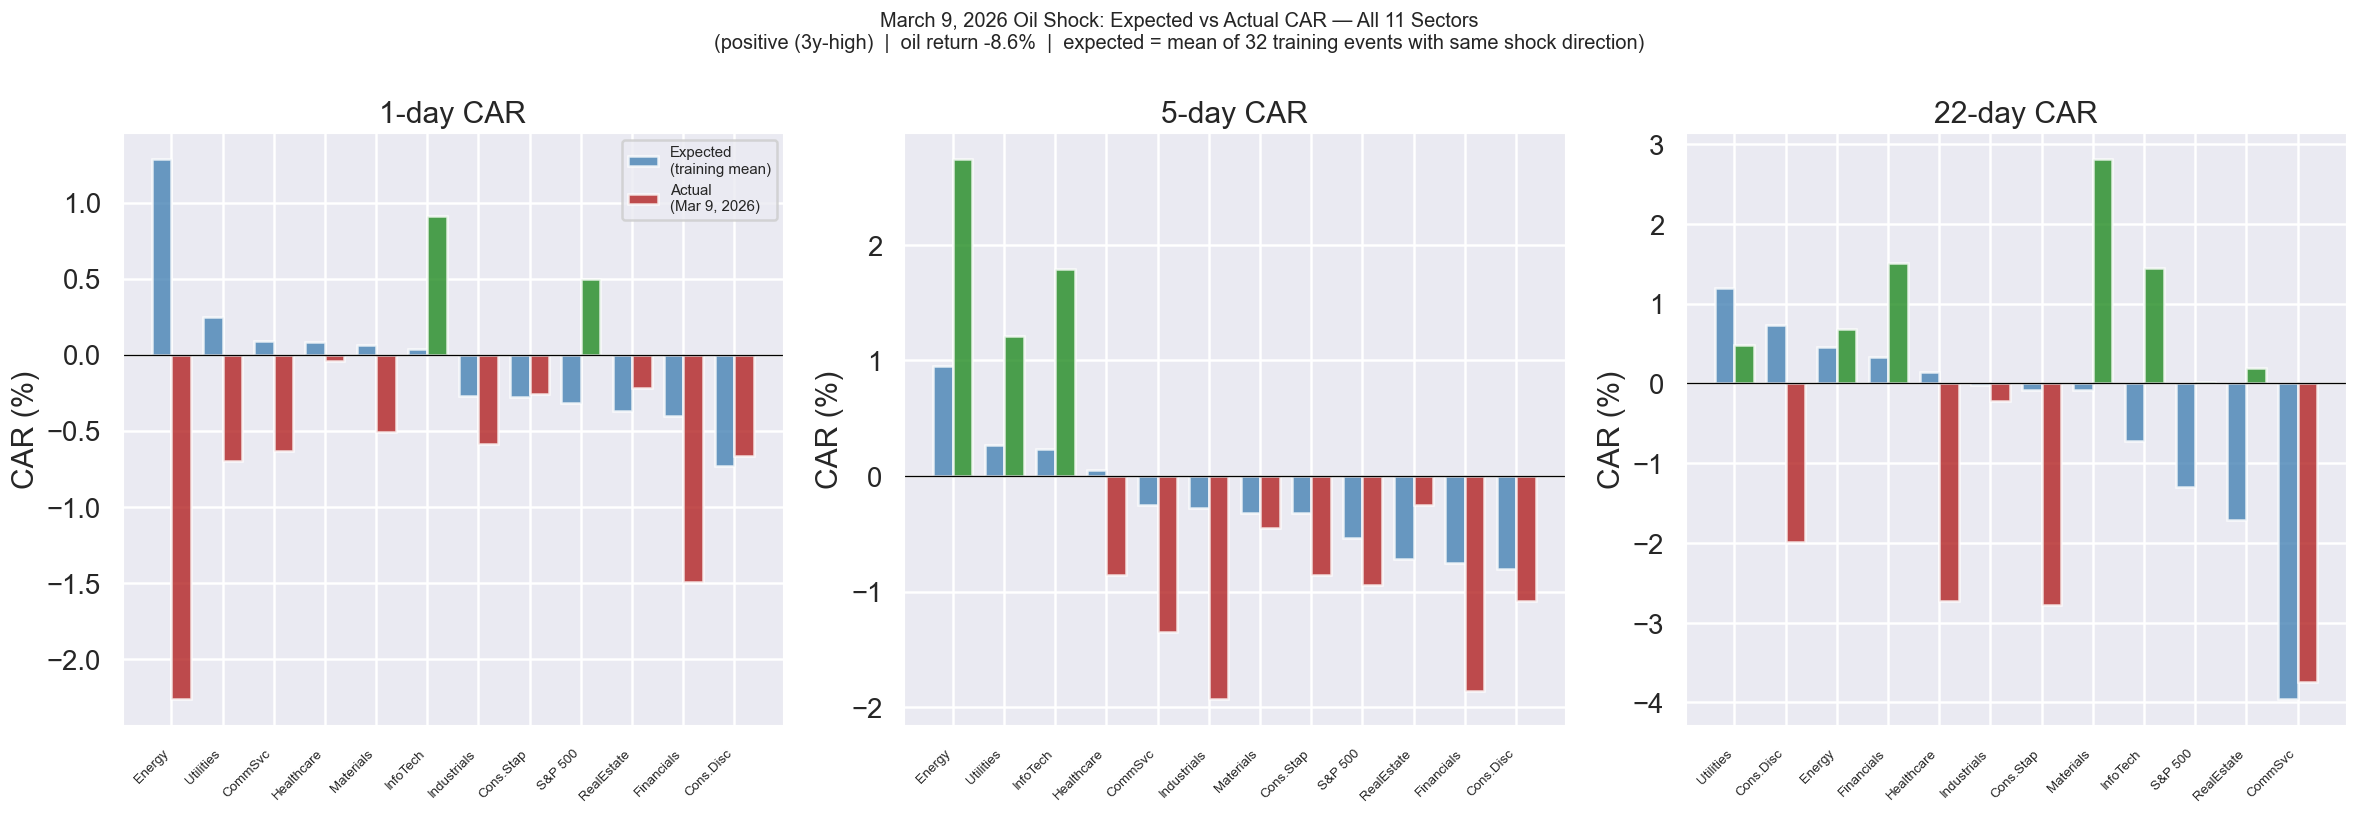
\includegraphics[width=\textwidth]{plots_event_study/2026_sector_comparison.png}
\caption{Expected vs.\ actual sector CARs for the March~9, 2026 oil shock. Expected = training-data mean CAR across 33 prior positive-shock events. Actual = observed post-event CAR. The 22-day window was dominated by tariff escalation and policy pivots.}
\label{fig:2026sectors}
\end{figure}

\begin{table}[H]
\centering
\caption{Full sector comparison: expected (training mean) vs.\ actual CARs. Entries in bold indicate direction-correct predictions.}
\label{tab:2026sectors}
\small
\begin{tabular}{lrrrrrr}
\toprule
Sector & Exp 1d & Act 1d & Exp 5d & Act 5d & Exp 22d & Act 22d \\
\midrule
S\&P 500 & $-0.32\%$ & $\mathbf{+0.50\%}$ & $-0.53\%$ & $-0.94\%$ & $-1.30\%$ & $+0.02\%$ \\
Energy (XLE) & $+1.28\%$ & $-2.27\%$ & $+0.95\%$ & $\mathbf{+2.74\%}$ & $+0.45\%$ & $\mathbf{+0.68\%}$ \\
Cons.\ Disc.\ & $\mathbf{-0.73\%}$ & $\mathbf{-0.67\%}$ & $-0.81\%$ & $-1.08\%$ & $+0.73\%$ & $-1.99\%$ \\
Info.\ Tech.\ & $+0.04\%$ & $\mathbf{+0.91\%}$ & $+0.23\%$ & $\mathbf{+1.79\%}$ & $-0.72\%$ & $+1.44\%$ \\
Healthcare & $+0.08\%$ & $-0.04\%$ & $+0.05\%$ & $-0.86\%$ & $+0.14\%$ & $-2.72\%$ \\
Cons.\ Staples & $\mathbf{-0.28\%}$ & $\mathbf{-0.26\%}$ & $-0.32\%$ & $-0.86\%$ & $-0.08\%$ & $-2.78\%$ \\
Financials & $-0.40\%$ & $-1.50\%$ & $-0.76\%$ & $-1.86\%$ & $+0.33\%$ & $\mathbf{+1.51\%}$ \\
Materials & $+0.06\%$ & $-0.51\%$ & $-0.32\%$ & $\mathbf{-0.45\%}$ & $-0.09\%$ & $\mathbf{+2.81\%}$ \\
Utilities & $+0.25\%$ & $-0.70\%$ & $+0.27\%$ & $\mathbf{+1.21\%}$ & $+1.20\%$ & $\mathbf{+0.48\%}$ \\
Real Estate & $-0.37\%$ & $\mathbf{-0.22\%}$ & $-0.72\%$ & $\mathbf{-0.25\%}$ & $-1.71\%$ & $+0.19\%$ \\
Comm.\ Svcs.\ & $+0.09\%$ & $-0.64\%$ & $-0.25\%$ & $-1.35\%$ & $\mathbf{-3.96\%}$ & $\mathbf{-3.75\%}$ \\
\bottomrule
\end{tabular}
\end{table}

\subsection{Cross-Sectional Model Predictions}

\begin{table}[H]
\centering
\caption{Cross-sectional model predictions vs.\ actuals for S\&P and XLE.}
\label{tab:2026models}
\begin{tabular}{llrrrr}
\toprule
Asset & Horizon & Actual & OLS & Ridge & Lasso \\
\midrule
S\&P & 1d  & $+0.50\%$ & $-0.67\%$ & $-0.88\%$ & $-0.83\%$ \\
S\&P & 22d & $+0.02\%$ & $-2.33\%$ & $-1.21\%$ & $-0.76\%$ \\
\midrule
XLE & 1d  & $-2.27\%$ & $\mathbf{-2.64\%}$ & $-0.28\%$ & $-1.91\%$ \\
XLE & 5d  & $+2.74\%$ & $-3.45\%$ & $+0.33\%$ & $+0.38\%$ \\
XLE & 22d & $+0.68\%$ & $+3.70\%$ & $+1.15\%$ & $+1.92\%$ \\
\bottomrule
\end{tabular}
\end{table}

\subsection{Interpretation}

\textbf{What the model got right.} (1)~Consumer Discretionary at 1d: $-0.73\%$ expected, $-0.67\%$ actual — near-exact match in direction and magnitude. (2)~Consumer Staples at 1d: $-0.28\%$ expected, $-0.26\%$ actual. (3)~Communication Services at 22d: $-3.96\%$ expected, $-3.75\%$ actual — remarkably accurate over the full month. (4)~OLS predicted XLE 1d to within 37~bp ($-2.64\%$ vs.\ $-2.27\%$).

\textbf{The key model failure: XLE 1d training-mean.} The training-mean prediction for XLE 1d was $+1.28\%$ (positive shock $\to$ energy benefits) vs.\ $-2.27\%$ actual. The market reacted to the \emph{daily return} ($-8.6\%$ on the day), not the price level classification. The cross-sectional OLS model that uses \texttt{ret\_oil} directly as a feature avoided this failure, confirming that \texttt{ret\_oil} is the correct 1-day predictor — not \texttt{shock\_dir}.

\textbf{22-day misses.} Healthcare ($-2.72\%$ actual vs.\ $+0.14\%$ expected), Materials ($+2.81\%$ vs.\ $-0.09\%$), Consumer Staples ($-2.78\%$ vs.\ $-0.08\%$) all show large deviations. The 22-day window was dominated by US tariff escalation and Federal Reserve policy pivot signals — macroeconomic forces entirely outside the model's feature set. This is consistent with the CV evidence that 22-day predictability is weak for all sectors.

%% ── 8. Robustness ─────────────────────────────────────────────────────────
\section{Robustness}
\label{sec:robustness}

\subsection{Alternative Shock Definition}
\label{sec:robustness_alt}

As a robustness check, we define shocks using a daily return threshold: $|\text{ret}_{\text{oil}}| > 3\sigma_{252}$ (three trailing standard deviations), with the same 22-day deduplication. This yields 71 events vs.\ 54 under the primary definition, with only 9 events overlapping ($\pm5$-day window). The secondary definition captures acute volatility spikes rather than gradual price regime changes.

\begin{table}[H]
\centering
\caption{Ridge CV $R^2$ comparison across shock definitions.}
\small
\begin{tabular}{lrrrr}
\toprule
Asset & H & Primary (3y extreme) & Secondary ($3\sigma$ spike) \\
\midrule
S\&P & 1d  & $-0.52$ & $\mathbf{-0.15}$ \\
S\&P & 5d  & $-0.20$ & $\mathbf{-0.12}$ \\
S\&P & 22d & $-0.35$ & $\mathbf{-0.23}$ \\
XLE & 1d  & $-0.01$ & $\mathbf{+0.10}$ \\
XLE & 5d  & $-0.37$ & $\mathbf{-0.05}$ \\
XLE & 22d & $-0.23$ & $\mathbf{-0.16}$ \\
\bottomrule
\end{tabular}
\end{table}

The secondary definition yields strictly better CV $R^2$ at every horizon and both assets. XLE 1d reaches $+0.10$ with only 5 features — positive Ridge CV $R^2$ — compared to $-0.01$ under the primary definition. The finding is consistent: acute daily volatility spikes have more immediate and predictable equity impacts than slow-moving price regime changes.

\subsection{Endogeneity of Demand/Supply Classifier}
\label{sec:robustness_endogeneity}

\texttt{shock\_type} ($= \operatorname{sign}(\text{ret}_{\text{oil}}) \times \operatorname{sign}(\text{ret}_{SP})$) is potentially endogenous — the S\&P return on the shock day is partly caused by the shock itself. We add a fully pre-determined analogue:
\[
\texttt{shock\_type\_lag} = \operatorname{sign}(\texttt{oil\_trend\_60}) \times \operatorname{sign}(\texttt{sp\_pre\_22})
\]
The two classifiers agree on 59.3\% of events. Ridge coefficients for both are heavily shrunk toward zero at all horizons, and main results are unchanged. The endogeneity concern does not materially affect conclusions.

%% ── 9. Limitations ────────────────────────────────────────────────────────
\section{Limitations and Future Work}

\begin{enumerate}[noitemsep]
  \item \textbf{Small sample.} 54 pre-2026 events is the binding constraint. Most CV $R^2$ are negative because signal-to-noise is insufficient to predict CAR magnitudes out-of-sample. Monthly data would yield more events per year at the cost of identification precision.

  \item \textbf{Causal identification.} A proper structural VAR decomposition \cite{kilian2009} on monthly data would provide cleaner demand/supply identification than the contemporaneous daily classifier used here.

  \item \textbf{Time-varying dynamics.} The US became a net oil exporter post-2015. The XLE--oil relationship may have structurally changed in the shale era. A Markov-switching or rolling-window model would test for structural breaks.

  \item \textbf{Single 2026 test event.} Only one event occurred before the data cutoff. Additional 2026 events will improve out-of-sample evaluation as the year progresses.
\end{enumerate}

%% ── 10. Conclusion ────────────────────────────────────────────────────────
\section{Conclusion}

We posed three empirical questions and provide the following answers.

\textbf{How do markets react to oil price shocks?} The aggregate S\&P~500 shows no consistent abnormal return. Sector responses are interpretable but dispersed: Energy outperforms on positive shocks; Consumer Discretionary and InfoTech underperform. The cause (demand vs.\ supply) shapes sector rotation more than the direction of the shock. PCA confirms that oil shocks transmit through at least three independent channels with no single dominant factor.

\textbf{What can we predict?} XLE's 1-day abnormal return is the most predictable target in the analysis, driven mechanically by \texttt{ret\_oil\_abs} and \texttt{sigma\_252}. RF and GBM achieve positive CV $R^2$ (+0.14, +0.21) at this horizon. S\&P direction is weakly predictable using extended features (Ridge\_ext beats the null at all horizons). All predictability evaporates by day 5 for XLE and by day 22 for S\&P.

\textbf{What did the 2026 event confirm?} The March~9, 2026 event validated all three core conclusions: S\&P 22d CAR was $+0.02\%$ (models predicted $-0.76\%$ to $-2.33\%$ — near-zero was the right call); OLS predicted XLE 1d to within 37~bp; 22-day sector outcomes were dominated by macroeconomic forces orthogonal to the oil-shock feature set.

%% ── References ────────────────────────────────────────────────────────────
\begin{thebibliography}{9}
\bibitem{hamilton1983}
Hamilton, J.D.\ (1983). Oil and the Macroeconomy since World War II.
\textit{Journal of Political Economy}, 91(2), 228--248.

\bibitem{kilian2009}
Kilian, L.\ \& Park, C.\ (2009). The Impact of Oil Price Shocks on the U.S.\ Stock Market.
\textit{International Economic Review}, 50(4), 1267--1287.
\end{thebibliography}

%% ── Appendix: Source Attribution ──────────────────────────────────────────
\appendix
\section{Source Attribution}
\label{app:attribution}

In accordance with course requirements, all data sources, software tools, and AI assistance used in this project are documented below.

\subsection{Data}

\begin{itemize}[noitemsep]
  \item \textbf{Brent crude prices:} FRED (Federal Reserve Bank of St.\ Louis), series \texttt{DCOILBRENTEU}. Downloaded April 2026.
  \item \textbf{Equity prices (SPDR sector ETFs, S\&P~500):} Yahoo Finance via \texttt{yfinance} Python package, adjusted daily close prices.
  \item \textbf{VIX:} Yahoo Finance, ticker \texttt{\^{}VIX}.
  \item \textbf{DXY (US Dollar Index):} Yahoo Finance, ticker \texttt{DX-Y.NYB}.
  \item \textbf{US Treasury yields:} FRED series \texttt{DGS10} (10-year) and \texttt{DTB3} (3-month).
\end{itemize}

\subsection{Software}

All analysis is implemented in Python 3.11. Key packages: \texttt{pandas}, \texttt{numpy}, \texttt{scikit-learn} (Ridge, Lasso, RandomForestRegressor, GradientBoostingRegressor, cross\_val\_score), \texttt{statsmodels} (OLS, quantile regression), \texttt{matplotlib}/\texttt{seaborn} (visualisation). Full source code is in \texttt{analysis.py}.

\subsection{LLM Assistance}

This project used \textbf{Claude Sonnet 4.6} (Anthropic) via the Claude Code CLI for the following tasks:

\begin{itemize}[noitemsep]
  \item Iterative code development and debugging of \texttt{analysis.py}: event study functions, CV loop, LOO backtest, PCA, quantile regression, and secondary shock definition robustness checks.
  \item Drafting and refining the textual write-up in \texttt{README.md} and this \LaTeX\ report.
  \item Interpreting model outputs and structuring the out-of-sample comparison (Section~\ref{sec:oos}).
\end{itemize}

\noindent Representative prompts included (abbreviated):
\begin{itemize}[noitemsep]
  \item \emph{``Add a robustness check using a $3\sigma$ daily return threshold as an alternative shock definition and compare CV $R^2$ across both definitions.''}
  \item \emph{``The null baseline CV $R^2$ is strongly negative; update the results tables and interpretation to evaluate models relative to the null, not zero.''}
  \item \emph{``Make \texttt{README.md} into a \LaTeX\ file according to the guidelines in \texttt{prompt.md}.''}
\end{itemize}

\noindent No LLM was used for data collection or to generate quantitative results; all numerical outputs derive from \texttt{analysis.py} executed on real data.

\end{document}
